% вторая часть
\section{Предложения по улучшению методики обработки данных}

\subsection{Проблемы существующего подхода}
Рассмотрев методику проведения процедуры КГО согласно\cite{RD} можно выделить несколько замечаний, которые можно пересмотреть:

1. Метод анализа данных, приведённый в параграфе 1.3, основывается на поиске выбросов по правилу "3 сигм". Данное правило утверждает, что  абсолютная величина отклонения нормально распределённой случайной величины от её математического ожидания не превосходит трёх среднеквадратичных отклонений с вероятностью\cite{KremerMatstat}:
\begin{equation} \label{eq:3sigma_rule}
	P(|X - m| < 3\sigma)  = 0,9973.
\end{equation}

Проблема этого метода заключается в том, что он применим для выборок, значения которых извлечены из нормально распределённых генеральных совокупностей. Но в случае проведения КГО(согласно разделу 1) нет достаточных оснований утверждать, что все значения активностей будут распределены по нормальному закону. Следовательно, требуется проверить характер распределения для каждой выборки с целью установления корректности применения метода "3 сигм".

Кроме того, среднее и среднеквадратическое отклонение, рассчитываемые в данном методе, также изменяются под воздействием аномальных значений, что приводит к маскировке выбросов\cite{emissions}. Следовательно, имеет смысл рассмотреть альтернативы, например метод межквартильного размаха(IQR).

2. Процедура КГО с учётом времени и объёма испытаний может проходить до нескольких недель. С течением времени в БВ, а также в воде, подаваемой на стенд КГО, может изменяться концентрация борной кислоты с целью борного регулирования, что негативно сказывается на однородности условий проведения испытаний. В связи с этим значения активностей ПД, полученные в разное время, могут принадлежать разным статистическим распределениям, следовательно, анализироваться должны отдельно. 

Согласно пункту 1.3.3, разделение на выборки происходит "На основании визуального анализа"\ графических данных. Хочу отметить, что в изучаемой методике существует способ анализа полученных выборок на принадлежность к одному статистическому распределению с целью объединения нескольких выборок, но он не учитывает анализ на корректность разбиения исходных данных. В связи с вышеперечисленным возникает необходимость проверки данных в выборках, полученных на основании визуального анализа.

3. Описанный процесс анализа данных производится в ручном режиме с использованием программного комплекса Excel. Автоматизация этого процесса позволит снизить вероятность ошибок, ведущих к преждевременной остановке реактора, а также снизить потребность во временных и трудовых затратах.

\subsection{Предложения по улучшению}

\subsubsection{Метод IQR}

Учитывая изложенное в 2.1.1, в качестве альтернативы методу "3 сигм"\ имеет смысл рассмотреть метод поиска выбросов с помощью межквартильного размаха(Interquartile range/IQR).

Межквартильный размах (IQR) — это статистическая мера, равная разности между первым и третьим квартилями распределения (25-м и 75-м процентилями). Первый квартиль (Q1) — это значение, ниже которого находится 25\% данных, а третий квартиль (Q3) — это значение, ниже которого находится 75\% данных. Можно так же сказать, что интерквартильный размах это половина выборки, центрированная относительно медианы. 

Этот показатель полезен для оценки изменчивости признака в асимметричных распределениях или наборах данных с выбросами. Интерквартильный размах является устойчивым(робастным) аналогом дисперсии, поскольку не подвержен влиянию аномальных значений. Именно поэтому он является наиболее перспективным аналогом методу "3 сигм". 
Таким образом, интерквартильный размах позволяет обнаруживать аномальные значения, являясь альтернативой среднеквадратическому отклонению, которое эффективно только для нормально распределенных данных. IQR — это непараметрическая оценка, что делает его применимым для анализа данных любого распределения.

В современных практиках поиска выбросов с использованием межквартильного размаха применяется следующий метод расчёта критических значений:
\begin{equation} \label{eq:IQRmin}
	X^{min}  = Q1-1.5*IQR;
\end{equation}

\begin{equation} \label{eq:IQRmax}
	X^{max}  = Q3+1.5*IQR;
\end{equation}


На рисунке~\ref{fig:ris6} приведена иллюстрация коэффициента IQR для нормального распределения.

\begin{figure}[H]
	\centering
	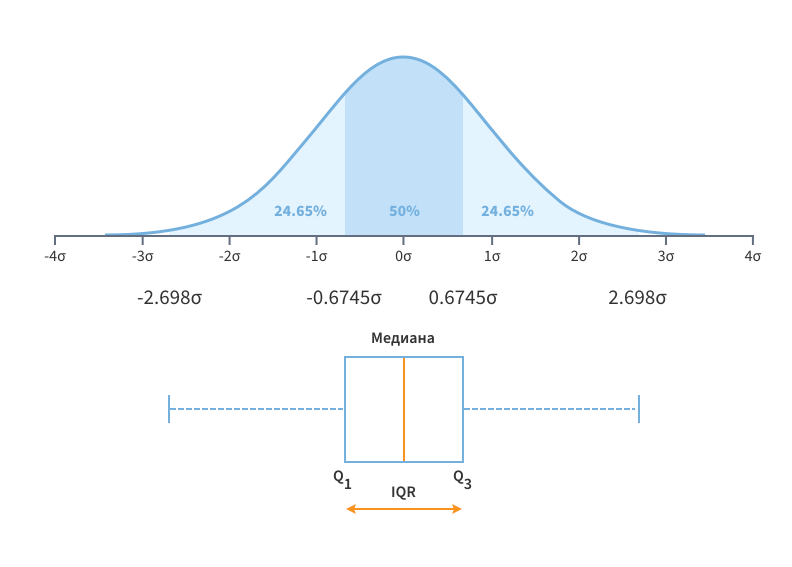
\includegraphics[width=1\linewidth]{pics/ris6} % изображения хранятся в подкаталоге pics
	\caption{Графическое представление межквартильного размаха на примере нормального распределения.}
	\label{fig:ris6} % эта метка позволяет ссылаться на рисунок в тексте
\end{figure}

Из рисунка~\ref{fig:ris6} видно, что данный подход в случае нормального распределения охватывает интервал:
\begin{equation} \label{eq:IQRP}
	P(|X^{min/max} - X| < 2.698\sigma)  = 0,9545.
\end{equation}

%Использование этого метода в качестве альтернативы методу "3 сигм"\ с точностью, требуемой в условии \ref{eq:3sigma_rule}, требует замену коэффициента при IQR в формулах~\ref{eq:IQRmin}-\ref{eq:IQRmax}.

%\begin{equation} \label{eq:IQR}
%	P(Q3+1.7*IQR - X < 3\sigma)  = 0,9973
%\end{equation}

\subsubsection{Критерий Шапиро-Уилка}
Как было описано выше, применение метода "3 сигм" обосновано в случаях, когда распределение выборки близко к нормальному. Следовательно, требуется установить насколько сильно анализируемое распределение отклоняется от нормального закона.
На основании результата данной проверки принимается решение относительно выбора метода поиска выбросов. 

В качестве критерия проверки распределения на нормальность был выбран критерий Шапиро-Уилка. Данный критерий был выбран на основании его мощности для выборок низкого объёма(8<n<50)\cite{Shapiro}.

Критерий Шапиро–Уилка, базируется на анализе линейной
комбинации разностей ранговых статистик. При построении статистики для вариационного ряда $ X_{(1)} \leq X_{(2)} \leq X_{(3)} \leq X_{(4)} \leq ... \leq X_{(n)}, $ полученного по наблюдаемой выборке $X_{1}, X_{2}, ... , X_{n}$, вычисляют величину\cite{RANstat}:

\begin{equation} \label{eq:Shapiro_S}
	S = \sum_{k}\alpha_{k}[X_{(n+1-k)} - X_{(k)}],
	%\frac{A_{j,кго}^{^{134}Cs}}{A_{j,кго}^{^{137}Cs}}
\end{equation}
где индекс k изменяется от 1 до n/2 или от 1 до (n - 1)/2 при четном и нечетном n соответственно. Коэффициенты $\alpha_{k}$ a приведены в~\cite{Shapiro}.
Статистика критерия вычисляется по формуле:

\begin{equation} \label{eq:Shapiro_W}
	W = \frac{S^2}{\sum_{i-1}^{n}(X_{i}-\overline{X})^2}.
\end{equation}

Таблица критических значений p-квантилей для статистики W приводятся в \cite{shapiro_GOST}.

Данный критерий проверяет следующие гипотезы:
\begin{itemize}
	\item Гипотеза H$_{0}$: "Cлучайная величина X распределена нормально".
	\item Гипотеза H$_{1}$: "Распределение случайной величины X не соответствует нормальному закону". 
\end{itemize}

% 3. Исходя из изложенного в 1.3.1-1.3.2 требуется разделять исходные данные на выборки, принадлежащие как минимум одному статистическому распределению, в идеальном случае требуется, чтобы выборка подчинялась нормальному закону распределения.